%
% chapter.tex -- Numerik der partiellen Differentialgleichungen
%
% (c) 2025 Prof Dr Andreas Müller
%
\chapter{Numerik der partiellen Differentialgleichungen
\label{chapter:pdenumerik}}
\kopflinks{Numerik der partiellen Differentialgleichungen}
Feldgleichungen sind typischerweise partielle Differentialgleichungen,
die nur in den seltensten Fällen in geschlossener Form lösbar sind.
Die allgemeine Theorie der partiellen Differentialgleichungen kann
zwar Antwort geben auf die Frage nach den Anforderungen an die
Randbedingungen erforderlich sind, damit
die Lösungen eindeutig bestimmt sind. 
Um die Lösung zu bestimmen, bleiben somit nur numerische Methoden.
In diesem Kapitel sollen ein paar Grundideen vermittelt werden, die
auf alle Arten von partiellen Differentialgleichungen anwendbar sind.
Die Kapitel~\ref{chapter:neuronal},
\ref{chapter:openfoam},
\ref{chapter:parallelisierung}
und
\ref{chapter:reynolds}
geben einen Einblick in die vielfältigen Techniken, die zur Lösung
von speziellen Feldgleichungen entwickelt wurden.

Allen Verfahren gemeinsam ist die Notwendigkeit einer Diskretisierung.
Statt die gesuchten Funktion in ihrer Gesamtheit zu bestimmen, wird sie
durch Zahlenwerte angenährt, die für einen einzelnen Punkt
(finite Differenzen, Abschnitt~\ref{buch:pdenumerik:section:fdm}),
für einzelne Teilgebiete des Definitionsbereichs
(finite Volumina, Abschnitt~\ref{buch:pdenumerik:section:fvm})
oder für eine Frequenz oder Wellenzahl (Spektrale Methoden,
Abschnitt~\ref{buch:pdenumerik:section:spektral})
repräsentativ sind.
Die in Abschnitt~\ref{buch:pdenumerik:section:fem} skizzierte
Methode der finiten Elemente ersetzt die Funktion teilgebietweise
durch Polynome oder andere einfach auswertbare Funktionen.

Das Resultat der Diskretisierung ist eine Menge von algebraischen
Gleichungen für eine typischerweise sehr grosse Zahl von Unbekannten.
Für lineare Differentialgleichungen sind die algeraischen Gleichungen
ebenfalls linear.
Die Anzahl der Variablen ist leider meistens so gross, dass der
wohlbekannte gausssche Eliminationsalgorithmus mit seiner
$O(n^3)$-Komplexität viel zu langsam ist.
Es müssen daher auch neue Algorithmen zur Lösung der linearen
Gleichungssysteme gefunden werden, die die speziellen Eigenschaften
der durch Diskretisation entstandenen Gleichungen ausnützen können.


%
% Finite Differenzen
%
\section{Finite Differenzen
\label{buch:pdenumerik:section:fdm}}
Die einfachste Methode, Differentialgleichungen zu diskretisieren,
ist nur Funktionswerte in diskreten Punkten zu betrachten und die
Differentialquotienten durch Differenzenquotienten zu approximieren.
Dies ist die Methode der finiten Differenzen.
\index{finite Differenz}%
\index{Differenzen, finite}%

%
% Differenzenquotienten in einer Dimension
%
\subsection{Differenzenquotienten in einer Dimension
\label{buch:pdenumerik:fdm:subsection:1d}}
Für die Differentialgleichung $y''=0$ auf dem Intervall $[a,b]$
zum Beispiel können wir die Funktion auf die äquidistanten Punkte
%
% fig-1d.tex
%
% (c) 2025 Prof Dr Andreas Müller
%
\begin{figure}
\centering
\vspace*{2cm}
XXX
\vspace*{2cm}
\caption{Diskretisation mit finiten Differenzen in einer Dimension
\label{buch:pdenumerik:fdm:fig:1d}}
\end{figure}
%
\[
x_0=a,
x_1=h,
x_2=2h,
\dots
x_{n-1}=(n-1)h,
x_n=b
\]
mit Schrittweite $h = (b-a)/n$ einschränken, wie dies in
Abbildung~\ref{buch:pdenumerik:fdm:1d} gezeigt ist.
Wir bezeichnen die Funktionswerte mit $y_k = y(x_k)$.
Die Ableitung an der Stelle $x_k$ kann dann durch den Differenzenquotienten
\[
y'(x_k)
\approx
\frac{\Delta y}{\Delta x}
=
\frac{y_{k+1}-y_k}{h}
\]
approximiert werden.
Und die zweite Ableitung ist
\[
y''(x_k)
\approx
\frac{y'(x_k) - y'(x_{k-1})}{h}
=
\frac{(y_{k+1}-y_{k})-(y_k-y_{k+1})}{h^2}
=
\frac{y_{k+1}-2y_{k}-y_{k+1}}{h^2}.
\]
Die Differentialgleichung $y''=0$ wird daher zu einem System von
linearen Gleichung
\[
y_{k+1} - 2y_k + y_{k-1} = 0
\]
für $k=1,\dots,n-1$.

%
% Diskretisierter Laplace-Operator in zwei Dimensionen
%
\subsection{Diskretisierter Laplace-Operator in zwei Dimensionen
\label{buch:pdenumerik:fdm:subsection:laplace}}
Auch für den zweidimensionalen Laplace-Operator wie in der Gleichung
$\Delta u = f$ kann eine analoge Diskretisation durchgeführt
werden.
%
% fig-2d.tex
%
% (c) 2025 Prof Dr Andreas Müller
%
\begin{figure}
\centering
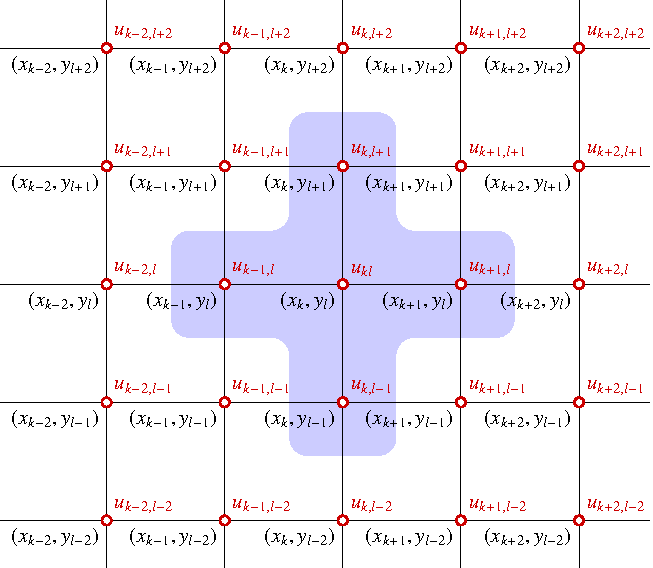
\includegraphics{chapters/090-pdenumerik/images/2d.pdf}
\caption{Diskretisation mit finiten Differenzen in zwei Dimension.
Für jeden Gitterpunkt wird einen Variable ({\color{darkred}rot}) benötigt.
Für die Berechnung einer Approximation des Laplace-Operators an der
Stelle $(x_k,y_l)$ sind die Variablen im blauen Kreuz notwendig.
\label{buch:pdenumerik:fdm:fig:2d}}
\end{figure}
%
Für ein Gitter von Punkten $(x_k,y_l) = (kh,lh)$ mit Schrittweite $h$
wie in Abbildung~\ref{buch:pdenumerik:fdm:fig:2d}
schreiben wir $u_{kl}=u(x_k,y_l)$ für die Werte der Lösungsfunktion.
Die Ableitungen können dann wieder durch die Differenzenquotienten
\begin{align*}
\frac{\partial u}{\partial x}(x_k,y_k)
&\approx
\frac{u_{k+1,l}-u_{kl}}{h}
&
\frac{\partial u}{\partial y}(x_k,y_k)
&\approx
\frac{u_{k,l+1}-u_{kl}}{h}
\\
\frac{\partial^2 u}{\partial x^2}(x_k,y_k)
&=
\frac{u_{k+1,l}-2u_{kl}+u_{k-1,l}}{h^2}
&
\frac{\partial^2 u}{\partial x^2}(x_k,y_k)
&=
\frac{u_{k,l+1}-2u_{kl}+u_{k,l-1}}{h^2}
\end{align*}
approximieren.
Die Differentialgleichung wird dann durch die lineare Gleichung
\[
\Delta u(x_k,y_k)
\approx
\frac{1}{h^2}
\bigl(
u_{k+1,l}+u_{k-1,l}+u_{k,l+1}+u_{k,l-1} - 4 u_{kl}
\bigr)
=
f_{kl} = f(x_k,y_l)
\]
ersetzt.


%
% Finite Volumina
%
\section{Finite Volumina
\label{buch:pdenumerik:section:fvm}}

%
% Finite Elemente
%
\section{Finite Elemente
\label{buch:pdenumerik:section:fem}}
Die Methode der finiten Differenzen verwendet die Funktionswerte
in den Gitterpunkten, um die Ableitungen durch Differenzenquotienten
zu approximieren.
Dies entspricht einer linearen Approximation der Funktion zwischen
den Gitterpunkten.
Die Methode der finiten Elemente versucht, die Werte in den
Gitterpunkten dazu zu verwenden, eine Approximation der Lösungsfunktion
zu konstruieren, die auch zwischen den Gitterpunkten eine gut ist.
Sie kann zusätzlich auch Ableitungswerte in den Gitterpunkten als
Unbekannte verwenden.
Die Konstruktion der linearen Gleichungen wird etwas komplizierter,
sie verwendet Integrale über die Intervalle oder Gebiete zwischen
den Gitterpunkten.
Dies ermöglicht, eine sehr gute Approximation mit einer vergleichsweise
kleinen Zahl von Gitterpunkten zu konstruieren.

%
% Schwache Form der Differentialgleichung
%
\subsection{Schwache Form der Differentialgleichung}
Zur Illustration der Idee der Methode der finiten Elemente verwenden wir
als Beispiel die eindimensionale Differentialgleichung
\begin{equation}
u''(x) = f(x)
\label{buch:pdenumerik:fem:eqn:u2}
\end{equation}
auf dem Intervall $[a,b]$.
Dies ist der eindimensionale Fall der Laplace-Gleichung $\Delta u = f$.

%
% Skalarprodukt
%
\subsubsection{Skalarprodukt}
Die Gleichung \eqref{buch:pdenumerik:fem:eqn:u2} ist gleichbedeutend
mit $u''(x)-f(x)=0$.
Es geht also darum, Bedingungen aufzustellen, die garantieren können,
dass $u''(x()-f(x)=0$ ist.
Eine Analogie zur Vektorgeometrie kann helfen zu verstehen, wie dies 
gelingen kann.
Ein Vektor $\vec{v}\in\mathbb{R}^n$ verschwindet, wenn jede einzelne
Komponente $=0$ ist.
Das ist die lokale Betrachtungsweise der Methode der finiten Differenzen.
Man kann aber auch eine beliebige Basis $\vec{b}_1,\dots,\vec{b}_n$ nehmen
und als Bedingung stellen, dass 
\[
\vec{v}\cdot\vec{b}_k = 0
\]
ist für $k=1,\dots,n$.

Auf die Gleichung \eqref{buch:pdenumerik:fem:eqn:u2} übertragen
bedeutet dies, dass wir zunächst ein Skalarprodukt für Funktionen
auf dem Intervall $[a,b]$ benötigen.
Das $L^2$-Skalarprodukt
\[
\langle f,g\rangle
=
\int_a^b f(x)g(x)\,dx
\]
bietet sich hier für an.
Dieses Skalarprodukt lässt sich auch für
ein beliebiges kompakte Gebiet $G\subset\mathbb{R}^n$ definieren.

Als nächstes wird eine Familie $g_i(x)$ von Funktionen benötigt, mit
denen man die Bedinungen $\langle u''-f,g_i\rangle=0$
formulieren kann.
Und schliesslich braucht es eine Approximationsfunktion für $u$, die zweimal
differenzierbar ist und für die man das Skalarprodukt berechnen kann.

%
% Reduktion der Ordnung mit partieller Integration
%
\subsubsection{Reduktion der Ordnung mit partieller Integration}
Die gesuchten Approximationsfunktion, aus denen eine Approximation von
$u(x)$ zusammengebaut werden kann, scheinen zweimal stetig differenzierbar
sein zu müssen, damit $\langle u''-f,g_i\rangle$ überhaupt definiert ist.
Wenn die Funktionen $g_i$ stetig differenzierbar sind, dann kann man
mit partieller Integration das Skalarprodukt
\begin{align*}
\langle u'',g_i \rangle
&=
\int_a^b u''(x)g_i(x)\,dx
\\
&=
\Bigl[ u'(x) g_i(x) \Bigr]_a^b
-
\int_a^b u'(x) g'_i(x)\,dx
\\
&=
\Bigl[ u'(x) g_i(x)\Bigr]_a^b
-
\langle u', g'_i\rangle
\end{align*}
umwandeln.
Dieser Ausdruck ist wohldefiniert selbst wenn die Funktionen $u$ und $g_i$
nur einmal stetig differenzierbar sind.

%
% Schwache Form der Gleichungen
%
\subsubsection{Schwache Form der Gleichungen}
Wir nehmen jetzt an, dass die Funktion $u(x)$ als Linearkombination
\[
u(x) 
=
\sum_{k=1}^n a_k h_k(x)
\]
der Funktionen $h_i(x)$, mit $i=1,\dots,n$ geschrieben werden kann.
Setzt man diesen Ansatz in die Bedingung $\langle u''-f,g_i\rangle=0$ ein,
findet man
\begin{align}
\langle u''-f,g_i\rangle
=
\sum_{k=1}^n
u_k
\Bigl[h'_k(x) g'_i(x)\Bigr]_a^b
-
\sum_{k=1}^n
u_k
\langle h'_k,g'_i\rangle
-
\langle f,g_i\rangle
&=
0
\notag
\\
\sum_{k=1}^n
\Bigl(
\underbrace{
\bigl[h'_k(x)g'_i(x)\bigr]_a^b
-
\langle h'_k,g'_k\rangle
}_{\displaystyle =  a_{ik}}
\Bigr)
{\color{darkred}u_k}
&=
\langle f,g_i\rangle.
\label{buch:pdenumerik:fem:eqn:gleichungen}
\end{align}
Dies ist ein lineares Gleichungssystem für die Unbekannten $u_k$
mit der Koeffizientenmatrix $a_{ik}$ und rechten Seiten
$\langle f,g_i\rangle$.
Es kann aufgestellt werden, sobald die Funktion $g_i$ und $h_k$ festgelegt
sind.

%
% Approximationsfunktionen
%
\subsection{Approximationsfunktionen}
Zur erfolgreichen Durchführung der Methode der finiten Elemente
werden zwei Familien von Funktionen $g_i$ und $h_k$ benötigt.
Damit die Lösung der Gleichungen effizient wird, sollten die 
Funktionen sehr kleinen Träger haben, so dass nur jeweils wenige
Paare von Funktion $h'_k$ und $g'_i$ nichtverschwindendes Skalarprodukt
haben.

\subsubsection{Lineare Elemente}
Damit die Resultate einfach interpretiert werden können, sollte es
einen einfachen Zusammenhang zwischen den Koeffizienten $a_k$ und
den Funktionswerten geben.
Besonders leicht wird dies, wenn die $a_k$ wieder Funktionswerte
von $u$ auf den Punkten eines Gitters wie im
Abschnitt~\ref{buch:pdenumerik:fdm:subsection:1d} sind.
%
% fig-linear.tex
%
% (c) 2025 Prof Dr Andreas Müller
%
\begin{figure}
\centering
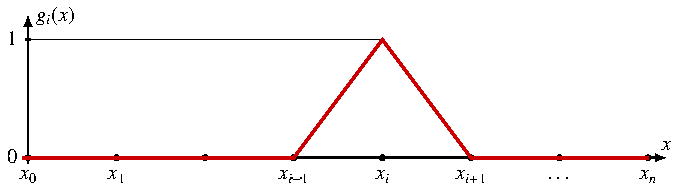
\includegraphics{chapters/090-pdenumerik/images/linear.pdf}
\caption{Die stückweise linearen Approximationsfunktionen $g_i(x)$
sind genau im Gitterpunkt $x_i$ von $0$ verschieden, wo der Wert $1$ ist,
und verschwinden in allen anderen Gitterpunkten.
\label{buch:pdenumerik:fem:fig:linear}}
\end{figure}
%
Die stückweise linearen Funktionen
\[
g_i(x_l) = \begin{cases}
1&\qquad i=l \\
0&\qquad i\ne l,
\end{cases}
\]
die auch in Abbildung~\ref{buch:pdenumerik:fem:fig:linear}
dargestellt sind.
Diese Funktionen können auch für die $h_k$ verwendet werden.

\subsubsection{Kubische Elemente}
Für die Differentialgleichung sind aber auch noch die 
Ableitungen der Funktionen nötig.
%
% fig-kubisch.tex
%
% (c) 2025 Prof Dr Andreas Müller
%
\begin{figure}
\centering
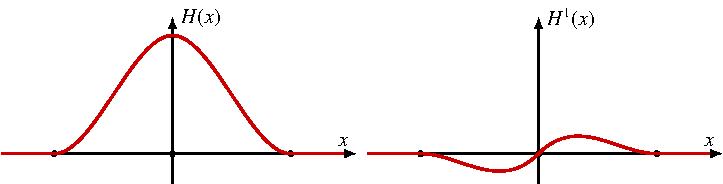
\includegraphics{chapters/090-pdenumerik/images/kubisch.pdf}
\caption{Kubische Approximationsfunktionen für die Methode der
finiten Elemente in einer Dimension.
Für ganzzahlige Argumente (schwarze Punkte auf der $x$-Achse)
hat die Funktion $H(x)$ nur bei $x=0$ den Wert $1$, alle anderen
Funktionswerte und alle Ableitungen verschwinden.
Die Funktion $H^1(x)$ ist in allen Gitterpunkten ebenso wie
ihre Ableitung $=0$ mit Ausnahme des Punktes $x=0$, wo die
Ableitung $=1$ ist.
\label{buch:pdenumerik:fem:fig:kubisch}}
\end{figure}
%
Die kubischen Funktionen 
\[
g_i(x)
=
H\biggl(\frac{x-x_i}{h}\biggr)
\qquad\text{mit} \qquad
H(x)
=
\begin{cases}
(1-2x)(1+x)^2    &\qquad -h\le x \le 0\\
(1+2x)(1-x)^2    &\qquad 0\le x \le h\\
0                &\qquad\text{sonst,}
\end{cases}
\]
die auch in Abbildung~\ref{buch:pdenumerik:fem:fig:kubisch}
dargestellt sind, sind stetig differenzierbar, haben aber
in den Gitterpunkten verschwindende Ableitungen, sie können daher
die Ableitungen der Lösungsfunktion nicht wiedergeben.

Nimmt man aber noch die Funktionen
\[
g^1_i(x)
=
hH^1(x)
\qquad\text{mit}\qquad
H^1\biggl(\frac{x-x_i}{h}\biggr)
=
\begin{cases}
x(1+x)^2         &\qquad -h\le x \le 0\\
x(1-x)^2         &\qquad 0\le x \le h\\
0                &\qquad\text{sonst}
\end{cases}
\]
hinzu, die ebenfalls in Abbildung~\ref{buch:pdenumerik:fem:fig:kubisch}
dargestellt sind, dann können auch Ableitungen wiedergegeben werden.
Die Funktionen $g_i^1$ haben nämlich im Punkte $x_i$ die Ableitung
\[
g^{1\prime}_i(x)\big|_{x=x_i}
=
H^{1\prime}(x)\big|_{x=0}
=
\bigl(
(1+x)^2+2x(1+x)
\bigr)\big|_{x=0}
=
1,
\]
während die Funktionswerte überall $=0$ sind.
Mit den zwei Funktionenfamilien $g_i$ und $g^1_i$ ist es jetzt
besonders einfach, die Funktionen $u(x)$ und $f(x)$ zu approximieren.
Wir schreiben dazu
\begin{equation}
u(x)
\approx
\sum_{i=1}^n \bigl(u(x_i) g_i(x) + u'(x_i) g_i^1(x)\bigr).
=
\sum_{i=1}^n \bigl(u_i g_i(x) + u'_i g_i^1(x)\bigr).
\label{buch:pdenumerik:fem:eqn:approx}
\end{equation}
Die Summe auf der rechten Seiten stimmt in den Gitterpunkten mit den
Funktionswerten und den ersten Ableitungen überein.
Auf die gleiche Art kann auch $f$ approximiert werden.

\subsubsection{Höhere Dimension}
Die bisher entwickelten Arten von Elementen sind jeweils entstanden
durch Translation und Skalierung der einfachen Funktionen $H(x)$ und
$H^1(x)$, die in diesem Zusammenhang auch \emph{Formfunktionen} genannt werden.
\index{Formfunktion}%
Die beiden Variablen $u_k$ und $u'_k$ in jedem Knoten des Gitters
bestimmen die Approximationsfunktion vollständig, sie heissen auch
die \emph{Knotenvariablen}.
\index{Knotenvariable}%

Jetzt da die Anforderungen an die Approximationsfunktionen etwas
klarer sind, können wir auch formulieren, wie die Formfunktionen
für die Ausdehnung der Methode auf höhere Dimensionen gestaltet sein
müssen.
Als Beispiel betrachten wir die Differentialgleichung 
\[
\Delta u = f
\]
auf einem Gebiet $G\subset\mathbb{R}^n$.
Der Einfachheit halber nehmen wir an, dass $u$ auf dem Rand $\partial G$
verschwinden soll, und verweisen für allgemeinere Randbedingungen auf
die Literatur.
Die Testfunktionen $v(x)$ werden daher so gewählt, dass sie auf dem
Rand verschwinden.
Die schwache Form der Gleichungen entsteht jetzt durch Multiplikation
mit einer ebenfalls auf $G$ definierten Testfunktion $v(x)$ und
Integration über das Gebiet:
\[
\langle \Delta u,v\rangle
=
\int_G \Delta u(x)\,v(x)\,dx
=
\int_G f(x) v(x)\,dx.
\]
Wegen $\Delta = \nabla\cdot\nabla$ kann das erste Integral mit
dem Satz von Gauss, angewendet auf die Divergenz 
\[
\operatorname{div} \bigl((\operatorname{grad} u )\, v\bigr)
=
(\operatorname{div}\operatorname{grad}u)\, v
+
\operatorname{grad u}\cdot\operatorname{grad}v
=
(\Delta u)\, v
+
\nabla u\cdot\nabla v
\]
umgewandelt werden in das Integral
\[
\langle \Delta u,v\rangle
=
\int_G \Delta u(x)\,v(x)\,dx
=
\int_{\partial G}
\nabla u(x)\, v(x)
\cdot d\vec{n}
-
\int_G
\nabla u(x)\cdot\nabla v(x)
\,dx.
\]
Das erste Integral verschwindet, weil die Testfunktion $v(x)$ auf
$\partial G$ verschwindet.
Es bleibt also nur noch das Integral von $\nabla u(x)\cdot\nabla v(x)$.

Der Gradient $\nabla u(x)$ ist durch die partiellen Ableitungen von $u(x)$
nach jeder einzelnen Koordinaten $x_i$, $i=1,\dots,n$ bestimmt.
Es sind also differenzierbare Formfunktionen mit der Eigenschaft
zu bestimmen, dass sie oder ihre partiellen Ableitungen in genau
einem Punkt des Gitters von $0$ verschieden sind.
In diesem Gitterpunkt sind die Funktionswerte $=1$ oder aber 
genau eine der partiellen Ableitungen.
Die Funktion $u(x)$ kann dann durch eine Linearkombination
dieser Formfunktionen approximiert werden, wobei die Koeffizienten
der Linearkombination genau der Funktionswert bzw.~die Werte
der partiellen Ableitungen in diesem Gitterpunkt sind.
Diese Variablen heissen wieder Knotenvariablen.

Es ist allerdings nicht nötig, ein quadratisches Gitter wie
in Abschnitt~\ref{buch:pdenumerik:fdm:subsection:laplace} zu verwenden.
Eine beliebige Triangulation des Gebietes ist auch denkbar.
Die Knotenvariablen sind dann die Werte der Funktion in einem Eckpunkt
der Triangulation und die Formfunktion verschwinden ausserhalb der Dreieck,
die diesen Eckpunkt nicht als Ecke haben.

%
% Lineare Gleichungen
%
\subsection{Lineare Gleichungen}
Mit der Approximation \eqref{buch:pdenumerik:fem:eqn:approx} der
Funktionen $u$ und $f$ können jetzt die linearen Gleichungen 
gemäss \eqref{buch:pdenumerik:fem:eqn:gleichungen} aufgestellt werden.
Dazu sind nur die Integrale
\[
\langle g_i,g_k\rangle,\quad
\langle g^1_i,g_k\rangle
\quad \text{und}\quad
\langle g^1_i,g^1_k\rangle
\]
zu berechnen, was dank der expliziten Form der Funktionen $H(x)$ und
$H^1(x)$ nur eine Fleissarbeit ist.

Die Vorgehensweise zur Aufstellung der linearen Gleichungen bleibt
in höheren Dimensionen unverändert.
Zu einer geeigneten Triangulation müssen erst Formfunktionen bestimmt
werden, die in genau einem Knoten einer Triangulation einen von 0
verschiedenen Wert oder eine von 0 verschiedene Ableitung haben.
Ausserdem soll der Träger in den angrenzenden Dreiecken der Triangulation
enhalten sein.
Das lineare Gleichungssystem hat dann als Koeffizienten die Skalarprodukte
von Funktionen Ableitungen.
Die Tatsache, dass die Träger der Funktionen sehr klein sind, führt
zu einer Koeffizientenmatrix, in der jeweils nur wenige Einträge
auf einer Zeile von 0 verschieden sind.
Solche Gleichungssysteme lassen sich mit den in
Abschnitt~\ref{buch:pdenumerik:section:linear} beschriebenen
iterativen Methoden sehr effizient lösen.


%
% Spektrale Methoden
%
\section{Spektrale Methoden
\label{buch:pdenumerik:section:spektral}}
Die Transformationsmethode zur Lösung partieller Differentialgleichungen
verwendet die Tatsache, dass Lösungsfunktionen immer als Reihe von
Eigenfunktionen des Laplace-Operators entwickelt werden können.
Zum Beispiel sind die Funktionen
\(
e_k(x) = e^{ikx}
\)
Eigenfunktionen des Ableitungsoperators auf dem Intervall $[0,2\pi]$,
denn es gilt
\[
\frac{d^2}{dx^2} e_k(x)
=
\frac{d^2}{dx^2} e^{ikx}
=
-k^2 e^{ikx}
=
-k^2 e_k(x).
\]
Der Eigenwert ist also $-k^2$.
Die Fourier-Theorie besagt, dass nicht allzu irreguläre periodische
Funktionen $f(x)$ als Reihe
\[
f(x)
=
\sum_{k\in\mathbb{Z}} c_ke^{ikx}
\]
geschrieben werden können.

Funktionen $f(\vartheta,\varphi)$ auf einer Kugeloberfläche können
ganz ähnlich als Funktionenreihe der sogenannten Kugelfunktionen
$Y^m_l(\vartheta,\varphi)$ geschrieben werden, die Eigenfunktionen
des Laplace-Operators sind:
\[
\Delta Y^m_l
=
-l(l+1) Y^m_l.
\]
Die ganzzahligen Werte von $l$ und $m$ erfüllen $|m|\le l$ und $l\ge 0$.

Als Beispiel für die Anwendung dieser Eigenschaften, nehmen wir an,
dass $f_n$ eine vollständige Familie von Eigenfunktionen des Laplace-Operators
mit Eigenwert $\lambda_n$ auf dem Gebiet $G$ ist. 
Jede Funktion $f$ auf dem Gebiet lässt sich also schreiben als
\begin{equation}
f = \sum_{k=1}^\infty a_k f_k.
\label{buch:pdenumerik:spektral:ansatz}
\end{equation}
Damit kann jetzt die Wärmeleitungsgleichung
\[
\frac{\partial f}{\partial t}
=
\kappa
\Delta f
\]
gelöst werden.
Setzt man den Ansatz~\eqref{buch:pdenumerik:spektral:ansatz} in die 
Differentialgleichung ein, ergibt sich
\[
\sum_{k=1}^\infty
\frac{d a_k}{d t}
f_k
=
\kappa \sum_{k=1}^n a_k \lambda_k f.
\]
Durch Koeffizientenvergleich für jedes $k$ folgt die gewöhnliche
Differentialgleichung
\[
\frac{d a_k}{d t}
=
\kappa \lambda_k a_k.
\]
Ihre Lösung ist $a_k(t) = a_k(0) e^{\lambda_kt}$.
Das schwierige Problem der Lösung der partiellen Differentialgleichung
wird durch den Ansatz~\eqref{buch:pdenumerik:spektral:ansatz} auf die
Lösung einer sehr einfachen gewöhnliche Differentialgleichung reduziert.

Die Idee lässt sich auch auf komplizierte, sogar nichtlineare
Feldgleichungen übertragen.
Es entstehen möglicherweise nichtlinear Differentialgleichungssysteme
für die Koeffizienten $a_k$.
In vielen Anwendungsfällen reicht eine vergleichsweise kleine Zahl
von Koeffizienten für eine gute Approximation der Lösung.
Diese sogenannten \emph{spektralen Methoden}
\index{spektrale Methode}%
werden zum Beispiel für die Berechnung der Strömungsfelder in der 
Erdatmosphäre vom Europäischen Zentrum für Mittelfristprognose
(ECMWF) verwendet.

Die Arbeit~\ref{chapter:fourier} von Martina Knobel und Gian Kraus
zeigt eine weitere Anwendung dieser Methoden.
Sie erklärt, wie spektrale Methoden eine Feldgleichung in eine Menge
unabhängiger quantenmechanischer Oszillatoren zerlegt, die als Quanten
eines Feldes betrachtet werden können.
In diesem Sinn sind die spektralen Methode die Grundlage für die
moderne Quantenfeldtheorie.

%
% Iterative Lösung linearer Gleichungssysteme
%
\section{Iterative Lösung linearer Gleichungssysteme
\label{buch:pdenumerik:section:linear}}
Die grosse Zahl der Variablen, die in diskretisierten Gleichungen auftreten,
macht den Gauss-Algorithmus ineffizient.
Ausserdem ist er besonders bei grossen Gleichungssystemen anfällig auf
Rundungsfehler.
Die folgenden iterativen Verfahren versuchen, eine ungefähre Lösung
schrittweise zu verbessern.
Sofern die Iterationsvorschrift stabil ist, ergibt sich die Unempfindlichkeit
auf Rundungsfehler automatisch daraus, dass kleine Fehler in späteren
Schritten ausgeglichen werden.
Für die nachfolgend skizzierten Verfahren kann man Kriterien angeben,
unter denen dies der Fall ist.

Im ganzen Abschnitt geht es um die Lösung eines linearen Gleichungssystems
der Form $Ax=b$ mit einer $n\times n$-Matrix $A\in M_n(\mathbb{R})$ und
einem $n$-dimensionalen Spaltenvektor $b\in\mathbb{R}^n$.
Für die nachfolgend diskutierten Verfahren nehmen wir an, dass die
Diagonalelemente $a_{kk}$ von $A$ alle von $0$ verschieden sind.

%
% Gauss-Seidel-Verfahren
%
\subsection{Gauss-Seidel-Verfahren
\label{buch:pdenumerik:linear:subsection:gauss-seidel}}
Das Verfahren von Gauss-Seidel geht davon aus, dass ein einzelne lineare
\index{Gauss-Seidel-Verfahren}%
Gleichung immer durch Modifikation einer Variable, deren Koeffizient in
der Gleichung nicht verschwindet, erfüllt werden kann.
Sie also
\begin{equation}
a_{k1}x_1 + \dots + a_{kk}x_k + \dots + a_{kn}x_n = b_k
\label{buch:pdenumerik:linear:gauss-seidel:eqn:gl}
\end{equation}
die $k$-te Gleichung des Gleichungssystems.
Wir nehmen ausserdem an, dass $a_{kk}\ne 0$ ist.
Dann kann man die Gleichung erfüllen, indem man für die Variablen $x_k$
den Wert
\begin{equation}
x_k^{\text{(neu)}}
=
\frac{1}{a_{kk}}
\biggl(
b_k
-
\sum_{i=1}^{k-1}a_{ki}x_i
-
\sum_{i=k+1}^na_{ki}x_i
\biggr)
\label{buch:pdenumerik:linear:gauss-seidel:eqn:schritt}
\end{equation}
wählt, den man durch Auflösen von
\eqref{buch:pdenumerik:linear:gauss-seidel:eqn:gl}
nach $x_k$ erhält.
Damit ist zwar Gleichung $k$ des Gleichungssystems erfüllt, aber über die
übrigen Gleichungen wissen wir nichts.
Unter noch zu bestimmenden Bedingungen kann man aber annehmen, dass 
$x_k^{\text{(neu)}}$ eine bessere Approximation der Lösung darstellt.

Aus dieser Idee lässt sich jetzt ein iteratives Verfahren konstruieren.
Wir beginnen mit einer initialen Schätzung $x^{(0)}$ der Lösung des
Gleichungssystems.
Ziel der Iteration ist, schrittweise bessere Approximationen $x^{(m)}$
der Lösung zu bestimmen, die gegen die Lösung $x$ konvergieren.

Um aus einer Approximation $x^{(m)}$ die nächste Iteration $x^{(m+1)}$
zu bestimmen, wenden wir die Lösungsformel der Reihe nach auf alle
Variablen an.
Die erste Variable wird ersetzt durch
\[
x_1^{(m+1)}
=
\frac{1}{a_{11}}
\biggl(
b_1
-
\sum_{i=2}^n a_{1i}x_i^{(m)}
\biggr).
\]
Für die Bestimmung von $x_2^{(m+1)}$ steht bereits ein neuer,
hoffentlich verbesserter Wert für $x_1$ zur Verfügung, daher wird
dieser in der Formel \eqref{buch:pdenumerik:linear:gauss-seidel:eqn:schritt}
verwendet.
Der neue Wert für $x_2$ ist daher
\begin{equation}
x_2^{(m+1)}
=
\frac{1}{a_{22}}
\biggl(
b_2 - a_{21}x_1^{(m+1)}
-
\sum_{i=3}^n a_{2i}x_i^{(m)}
\biggr).
\end{equation}
In jedem Schritt werden also die bereits neu berechneten Variablen
verwendet.
Für die Variable $x_k^{(m+1)}$ bekommen wir daher die allgmeine
Iterationsformel
\begin{equation}
x_k^{(m+1)}
=
\frac{1}{a_{kk}}
\biggl(
b_k - \sum_{i=1}^{k-1} a_{ki}x_i^{(m+1)} - \sum_{i=k+1}^n a_{ki}x_i^{(m)}
\biggr).
\label{buch:pdenumerik:linear:gauss-seidel:iteration}
\end{equation}

%
% Jacobi-Verfahren
%
\subsection{Jacobi-Verfahren
\label{buch:pdenumerik:linear:subsection:jacobi}}
Das Gauss-Seidel-Verfahren verbessert die Variablenwerte der Lösung
für eine Variable nach der anderen.
Dies bedeutet auch, dass die Berechnung nicht parallelisiert werden
kann.
Um $x_{k+1}^{(m+1)}$ zu berechnen, muss die Berechnung von $x_k^{(m+1)}$
bereits abgeschlossen sein.
Das Jaocbi-Verfahren löst dieses Problem, zum Preis einer langsameren
Konvergenz.

Statt bei der Anwendung der Formel
\eqref{buch:pdenumerik:linear:gauss-seidel:eqn:schritt}
die neuen Werte $x_i^{(m+1)}$ mit $i<k$ zu verwenden, verwenden wir
die bereits bekannten alten Werte $x_i^{(m)}$.
Als Iterationsformel verwenden wir daher
\begin{equation}
x_k^{(m+1)}
=
\frac{1}{a_{kk}}
\biggl(
b_k
-
\sum_{i=1}^{k-1} a_{ki} x_i^{(m)}
-
\sum_{i=k+1}^n a_{ki} x_i^{(m)}
\biggr)
=
\frac{1}{a_{kk}}
\biggl(
b_k
-
\sum_{i\ne k} a_{ki} x_i^{(m)}
\biggr).
\end{equation}
Die rechte Seite kann für alle $k$ parallel ausgewertet werden.

Die Anzahl der Rechenoperationen für einen Schritt des Jacobi-Verfahrens
ist für eine beliebige Matrix $n$ Multiplikationen und ebensoviele
Additionen für die Berechnung einer einzelnen Variable.
Für alle Variablen zusammen ist der Rechenaufwand also $O(n^2)$,
eine Potenz besser als für den Gauss-Algorithmus.

Matrizen $A$, die aus der Diskretisation einer partiellen
Differentialgleichung entstehen, enthalten in jeder Zeile nur ganz
wenige Einträge typischerweise von der Grössenordnung der
Dimension des Problems, unabhängig von $n$.
Dies bedeutet, dass der Rechenaufwand für die Neuberechnung
einer Variable tatsächlich nur von der Grössenordnung $O(1)$ ist
und damit für einen Schritt des Jacobi-Verfahrens $O(n)$, eine
wesentliche Verbesserung gegenüber dem gausschen Eliminationsalgorithmus.

%
% Matrix-Zerlegung
%
\subsection{Matrix-Zerlegung
\label{buch:pdenumerik:linear:subsection:matrix-zerlegung}}
Sowohl das Gauss-Seidel-Verfahren wie auch das Jacobi-Verfahren können
in Matrixform geschrieben werden, was erlaubt, für die Analyse der Konvergenz
des Verfahrens die Matrizenrechnung zu verwenden.
Das Gauss-Seidel-Verfahren zeigt, dass wir in der Formel
\eqref{buch:pdenumerik:linear:gauss-seidel:iteration}
die Matrixelement unterhalb der diagonalen jeweils mit den neuen
Variablenwerten $x_k^{(m+1)}$ und die Matrixelemente oberhalb der
Diagonalen mit den alten Weten $x_k^{(m)}$ verrechnet werden.
Wir zerlegen die Matrix $A$ daher in drei Matrizen:
\[
A = L + D + R,
\]
wobei $D$ die Diagonalelemente von $A$ umfasst, $L$ besteht aus den
Einträgen unterhalb der Diagonalen und $R$ aus den Einträgen oberhalb der
Diagonalen:
\[
L
=
\begin{pmatrix}
        0&        0&        0& \dots&        0&     0\\
   a_{21}&        0&        0& \dots&        0&     0\\
   a_{31}&   a_{32}&        0& \dots&        0&     0\\[-3pt]
   \vdots&   \vdots&   \vdots&\ddots&   \vdots&\vdots\\
a_{n-1,1}&a_{n-1,2}&a_{n-1,3}& \dots&        0&     0\\
   a_{n1}&   a_{n2}&   a_{n3}& \dots&a_{n,n-1}&     0
\end{pmatrix},
R
=
\begin{pmatrix}
     0&a_{12}&a_{13}& \dots&a_{1,n-1}&   a_{1n}\\
     0&     0&a_{13}& \dots&a_{2,n-1}&   a_{2n}\\
     0&     0&     0& \dots&a_{3,n-1}&   a_{3n}\\[-3pt]
\vdots&\vdots&\vdots&\ddots&   \vdots&   \vdots\\
     0&     0&     0& \dots&        0&a_{n-1,n}\\
     0&     0&     0& \dots&        0&        0
\end{pmatrix}
\]
und
\[
D
=
\operatorname{diag}(a_{11},\dots,a_{nn})
=
\begin{pmatrix}
a_{11}&     0& \dots&     0\\
     0&a_{22}& \dots&     0\\[-3pt]
\vdots&\vdots&\ddots&\vdots\\
     0&     0& \dots& a_{nn}
\end{pmatrix}
\]
Mit diesen drei Matrizen kann das Iterationsverfahren jetzt in
Matrixform geschrieben werden.

%
% Matrixform de Jacobi-Verfahrens
%
\subsubsection{Matrixform des Jacobi-Verfahrens}
Beim Jacobi-Verfahren werden gemäss
Formel~\ref{buch:pdelinear:jacobi:eqn:iteration} nur die alten
Werte verwendet, es gilt also
\[
Dx^{(m+1)} = b-(L+R)x^{(m)}
\qquad\Rightarrow\qquad
x^{(m+1)} = D^{-1}\bigl(b-(L+R) x^{(m)}).
\]
Dies ist die Iterationsformel für das Jacobi-Verfahren in Matrixform.

%
% Matrixform des Gauss-Seidel-Verfahrens
%
\subsubsection{Matrixform des Gauss-Seidel-Verfahrens}
Beim Gauss-Seidel-Verfahren werden die jeweils neu berechneten
Variablen verwendet, was durch die Gleichung
\[
(L+D)x^{(m+1)} = b-Rx^{(m)}
\]
ausgedrückt werden kann.
Die Iterationsformel des Gauss-Seidel-Verfahrens in Matrixform
ist daher
\[
x^{(m+1)} = (L+D)^{-1}(b - R x^{(m)}).
\]
Wegen $L+D=(LD^{-1}+I)D$ kann man $(L+D)^{-1}=D^{-1}(I+LD^{-1})^{-1}$
schreiben.
Dies scheint auf den ersten Blick sehr viel komplizierter, aber der
zweite Faktor kann mit Hilfe der neumannschen Reihe als
\[
(I+LD^{-1})^{-1}
=
I
- LD^{-1}
+ (LD^{-1})^2
- (LD^{-1})^3
+ (LD^{-1})^4
- \dots
=
\sum_{k=1}^\infty (-1)^k(LD^{-1})^k
\]
geschrieben werden.
Wenn $LD^{-1}$ kleine Operatornorm hat, dann konvergiert die Reihe
sehr rasch gegen die Inverse und der Ausdruck kann verwendet werden,
um für die nachfolgenden Konvergenzbetrachtungen eine Aussage über die
Operatornorm der Inversen zu bekommen.

%
% Konvergenz
%
\subsubsection{Konvergenz}
Für die Lösung des Gleichungssystems $Ax=b$ sind die Iterationsgleichungen
exakt erfüllt, es gilt also zum Beipsiel
\[
x
=
(L+D)^{-1}Rx
\qquad\text{ bzw. }\qquad
x
=
D^{-1}(L+R)x
\]
für das Gauss-Seidel- bzw.~das Jacobi-Verfahren.
Das Iterationsverfahren findet Approximationen von $x$, die wir als
\(
x^{(m)} = x + \delta x^{(m)}
\)
schreiben können.

Die Iterationsformel für das Jacobi-Verfahren wird damit zu
\begin{align*}
Dx^{(m+1)}
&=
b-(L+R)x^{(m)}
\\
Dx + D\delta x^{(m+1)}
&=
b - (L+R)x - (L+R)\delta x^{(m)}
\intertext{Da $x$ eine Lösung ist, gitl $Dx = b-(L+R)x$, so dass sich
die Gleichung zu}
D\delta x^{(m+1)}
&=
-(L+R)\delta x^{(m)}
\end{align*}
vereinfachen lässt.
Für den Fehler $\delta x^{(m)}$ gilt daher die einfachere
Jacobi-Iterationsformel
\[
\delta x^{(m+1)} = -D^{-1}(L+R)x^{(m)}.
\]
Für die Konvergenz des Verfahrens kommt es also ausschliesslich auf die
Eigenschaften der Matrix $D^{-1}(L+R)$ an.

Für das Gauss-Seidel-Verfahren liefert die analoge Rechnung
\begin{align*}
(L+D)x^{(m+1)}
&=
b - Rx^{(m)}
\\
(L+D)x + (L+D)\delta x^{(m+1)}
&=
b - Rx - R\delta x^{(m)},
\intertext{worin $(L+D)x=b-Rx$ vereinfacht werden kann, weil $x$ eine
Lösung ist.
Es bleibt die vereinfachte Gauss-Seidel-Iterationsformel}
(L+D)
\delta x^{(m+1)}
&=
-R\delta x^{(m)}
\\
\Rightarrow
\qquad
\delta x^{(m+1)}
&=
-(L+D)^{-1} R x^{(m)}
\end{align*}
für den Fehler.
Wieder können wir schliessen, dass es nur auf Eigenschaften der
Matrix $(L+D)^{-1}R$ ankommt.

In beiden Fällen haben wir gefunden, dass für den Fehler eine
Iterationsformel der Form $\delta x^{(m+1)} = C \delta x^{(m)}$
gilt.
Das Verfahren konvergiert für einen beliebigen Startwert genau dann,
wenn $\|C^n\|\to 0$ geht.
Dies ist der Fall, wenn der \emph{Gelfand-Radius}
\index{Gelfand-Radius}%
\[
\varrho(C)
=
\limsup_{n\to\infty} \|C^n\|^{\frac1n}
<
1
\]
ist.
Man kann zeigen, dass der Gelfand-Radius mit dem \emph{Spektralradius},
\index{Spektralradius}%
als mit dem Betrag des betragsgrössten Eigenwertes von $C$
übereinstimmt \cite{buch:linalg}.

\begin{satz}
Das Gauss-Seidel-Verfahren konvergiert genau dann, wenn der Spektralradius
von $(L+D)^{-1}R$ kleiner ist als $1$.
Das Jacobi-Verfahren konvergiert genau dann, wenn der Spetralradius von
$D^{-1}(L+R)$ kleiner ist als $1$.
\end{satz}

Die Bedingungen ist zum Beispiel dann erfüllt, wenn die Einträge auf
der Diagonalen viel grösser sind als die übrigen Einträge, die man in
$L$ und $R$ findet.

Aus dem Spektralradius kann man auch eine untere Schranke für die nötige
Anzahl der Iterationsschritte ableiten.
Wir nehmen dazu an, dass der Fehler zu Beginn die Grössenordnung
$\|\delta x^{(0)}\|=1$ hat
und durch die Iteration auf $\varepsilon$ verkleiner werden soll.
Die dazu nötige Anzahl Iterationen wird mit $m$ bezeichnet.
Der Fehler nach $m$ Iterationen ist
\[
\|\delta x^{(m)}\|
=
\| C^n \delta x^{(0)} \|
\le
\|C\|^m \|\delta x^{(0)}\|
=
\|C\|^m
\approx
\varrho(C)^m.
\]
Damit der Fehler kleiner $\varepsilon$ wird, muss $m$ so gross werden, dass
\begin{equation}
\varrho(C)^m < \varepsilon
\qquad\Rightarrow\qquad
m\log\varrho(C) < \log\varepsilon
\qquad\Rightarrow\qquad
m < \frac{\log\varepsilon}{\log\varrho(C)}.
\label{buch:pdenumerik:linear:konvergenzschritte}
\end{equation}

\begin{beispiel}
Für die Differentialgleichung $y''=0$ mit $n$ äquidistanten Punkten
führt auf die Matrix
\[
A
=
\begin{pmatrix}
    -4&     1&     0&     0& \dots &      0\\
     1&    -4&     1&     0& \dots &      0\\
     0&     1&    -4&     1& \dots &      0\\
     0&     0&     1&    -4& \dots &      0\\[-4pt]
\vdots&\vdots&\vdots&\vdots& \ddots& \vdots\\
     0&     0&     0&     0& \dots &     -4
\end{pmatrix}.
\]
Für die Konvergenz der beiden Iterationsverfahren sind die
Spektralradien der
von $C_{\text{Gauss-Seidel}}=(L+D)^{-1}R$ für das Gauss-Seidel-Verfahren
und
von $C_{\text{Jacobi}}=D^{-1}(L+R)$ für das Jacobi-Verfahren
bestimmen.
Die numerische Rechnung im Fall $n=2$ ergibt
\begin{align*}
\varrho(C_{\text{Gauss-Seidel}})
&\approx
0.9206
&&\text{bzw.}
&
\varrho(C_{\text{Jacobi}})
&\approx
0.9595.
\end{align*}
Beide Verfahren konvergieren also, auch wenn die Konvergenz nicht sehr schnell
ist.
Mit der Formel~\eqref{buch:pdenumerik:linear:konvergenzschritte}
kann auch die Anzahl Schritte für eine Verbesserung des Fehlers um den
Faktor $\varepsilon = 10^{-6}$ berechnet werden:
\begin{align*}
m_{\text{Gauss-Seidel}}
&=
167.05
&&\text{bzw.}&
m_{\text{Jacobi}}
&=
334.11.
\end{align*}
Die Anzahl der nötigen Iterationen für Konvergenz ist also sehr hoch.
\end{beispiel}



